\chapter{热学(选修3-3)}
\section{分子动理论 内能}

1.分子动理论的基本观点和实验依据、阿伏加德罗常数

(1)物体是由大量分子组成的

\ding{172}分子的大小

a.分子的直径(视为球模型):数量级为$10^{-10}$m;

b.分子的质量:数量级为$10^{-26} kg$.

\ding{173}阿伏加德罗常数

a.1
mol的任何物质都含有相同的粒子数.通常可取$\mathrm{N}_{\mathrm{A}}=6.02 \times 10^{23} \mathrm{mol}^{-1}$;

b.阿伏加德罗常数是联系宏观物理量和微观物理量的桥梁.

(2)分子永不停息地做无规则运动

\ding{172}扩散现象

a.定义:\_\_不同\_\_物质能够彼此进入对方的现象;

b.实质:扩散现象并不是外界作用引起的,也不是化学反应的结果,而是由分子的无规则运动产生的物质迁移现象,温度\_\_越高\_\_,扩散现象越明显.

\ding{173}布朗运动

a.定义:悬浮在液体中的\_\_小颗粒\_\_的永不停息地无规则运动;

b.实质:布朗运动反映了\_\_液体分子\_\_的无规则运动;

c.特点:颗粒越\_\_小\_\_,运动越明显,温度越\_\_高\_\_,运动越剧烈.

\ding{174}热运动

a.分子永不停息地做\_\_无规则\_\_运动叫做热运动;

b.特点:分子的无规则运动和温度有关,温度越高,分子运动越激烈.

(3)分子间同时存在引力和斥力

\ding{172}物质分子间存在空隙,分子间的引力和斥力是\_\_同时\_\_存在的,实际表现出的分子力是引力和斥力的\_\_合力\_\_;

\ding{173}分子力随分子间距离变化的关系:分子间的引力和斥力都随分子间距离的增大而\_\_减小\_\_,随分子间距离的减小而\_\_增大\_\_,但斥力比引力变化得\_\_快\_\_;

\ding{174}分子力与分子间距离的关系图线由分子间的作用力与分子间距离关系图线(如图所示)可知:

\begin{center}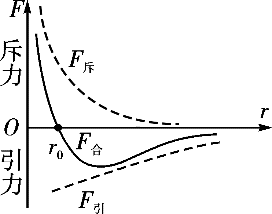
\includegraphics[width=1.23611in,height=0.97153in]{media/image485.png}\end{center}

a.当r$r=r_{0}$ 时 $, \quad F_{\text {引 }}=F_{F}$,分子力为\_\_零\_\_;

b.当$r>r_{0}$ 时 $, \quad F_{\text {引 }}=>F_{F}$,分子力表现为\_\_引力\_\_;

c.当$r<r_{0}$ 时 $, \quad F_{\text {引 }}<F_{F}$,分子力表现为\_\_斥力\_\_;

d.当分子间距离大于10$r_0$(约为$10^{-9} m$)时,分子力很弱,可以忽略不计.
\newpage
2.温度是分子平均动能的标志 内能

(1)温度

一切达到热平衡的系统都具有相同的\_\_温度\_\_.

(2)两种温标

摄氏温标和热力学温标.关系T=t+273.15 K.

(3)分子的动能

\ding{172}分子动能是\_\_分子热运动\_\_所具有的动能;

\ding{173}分子热运动的平均动能是所有分子热运动的动能的平均值,\_\_温度\_\_是分子热运动的平均动能的标志;

\ding{174}分子热运动的总动能是物体内所有分子热运动动能的\_\_总和\_\_.

(4)分子的势能

\ding{172}意义:由于分子间存在着引力和斥力,所以分子具有由它们的\_\_相对位置\_\_决定的能.

\ding{173}分子势能的决定因素

a.微观上:决定于\_\_分子间距离\_\_和分子排列情况,

b.宏观上:决定于\_\_体积\_\_和状态.

(5)物体的内能

\ding{172}概念理解:物体中所有分子的热运动\_\_动能\_\_与\_\_分子势能\_\_的总和,是状态量;

\ding{173}决定因素:对于给定的物体,其内能大小由物体的\_\_温度\_\_和\_\_体积\_\_决定,即由物体内部状态决定;

\ding{174}影响因素:物体的内能与物体的位置高低、运动速度大小\_\_无关\_\_.

\ding{175}改变物体内能的两种方式:\_\_做功\_\_和\_\_热传递\_\_.

\newpage
\subsection{微观量的估计}

1.求解分子直径时的两种模型(对于固体和液体)

(1)把分子看成球形,$\mathrm{d}=\sqrt[3]{\frac{6 \mathrm{V}_{0}}{\pi}}$.

(2)把分于看成小立方体,$\mathrm{d}=\sqrt[3]{\mathrm{V}_{0}}$

提醒:对于气体,利用$\mathrm{d}=\sqrt[3]{\mathrm{V}_{0}}$算出的不是分子直径,而是气体分于间的平均距离.

2.宏观量与微观量的相互关系

(1)微观量:分子体积$V_0$、分子直径d、分子质量$m_0$.

(2)宏观量:物体的体积V、摩尔体积Vmol、物体的质量m、摩尔质量M、物体的密度$\rho$.

(3)相互关系

\ding{172}一个分子的质量:$\mathrm{m}_{0}=\frac{\mathrm{M}}{\mathrm{N}_{\mathrm{A}}}=\frac{\rho \mathrm{V}_{\mathrm{mol}}}{\mathrm{N}_{\mathrm{A}}}$;

\ding{173}一个分子的体积:$V_{0}=\frac{V_{m o 1}}{N_{A}}=\frac{M}{\rho N_{A}}$;(注:对气体V0为分子所占空间体积)

\ding{174}物体所含的分子数:$\mathrm{n}=\frac{\mathrm{V}}{\mathrm{V}_{\mathrm{mol}}} \mathrm{N}_{\mathrm{A}}=\frac{\mathrm{m}}{\rho \mathrm{V}_{\mathrm{mol}}} \mathrm{N}_{\mathrm{A}}$ 或 $\mathrm{n}=\frac{\mathrm{m}}{\mathrm{M}} \mathrm{N}_{\mathrm{A}}=\frac{\rho \mathrm{V}}{\mathrm{M}} \mathrm{N}_{\mathrm{A}}$.

\begin{center}
\includegraphics[width=0.70764in,height=0.12292in]{media/image13.png}\end{center}
\begin{center}
    \textbf{微观量的求解方法}
\end{center}

(1)分子的大小、分子体积、分子质量属微观量,直接测量它们的数值非常困难,可以借助较易测量的宏观量结合摩尔体积、摩尔质量等来估算这些微观量,其中阿伏加德罗常数是联系宏观量和微观量的桥梁和纽带.

(2)建立合适的物理模型,通常把固体、液体分子模拟为球形或小立方体形.气体分子所占据的空间则建立立方体模型.

\newpage
\subsection{分子热运动与布朗运动}

布朗运动与分子热运动的比较

\begin{longtable}[]{@{}m{1.5cm}m{5cm}m{5cm}@{}}
\toprule
& 布朗运动 & 分子热运动\tabularnewline
\midrule
\endhead
共同点 &\multicolumn{2}{c}{都是无规则运动,都随温度的升高而变得更加剧烈} \tabularnewline
不同点 & 小颗粒的运动 & 分子的运动\tabularnewline
& 使用光学显微镜观察 & 使用电子显微镜观察\tabularnewline
联系 &\multicolumn{2}{l}{\shortstack{布朗运动是由于小颗粒受到周围分子热运动的撞击力而引起的,\\反映了分子做无规则运动}}\tabularnewline
\bottomrule
\end{longtable}

\subsection{分子与分子势能}

对分子势能的理解

分子势能与分子间的距离(宏观表现为物体的体积)有关,分子势能的大小随距离的变化如图所示,由图可知:

\begin{center}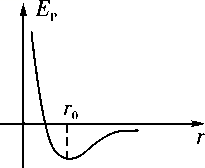
\includegraphics[width=0.93403in,height=0.76389in]{media/image487.png}\end{center}

1.当分子力为零时,即$r=r_0$时,分子势能不是零,而是最小.

2.当$r\textgreater r_0$时,分子力表现为引力,随着分子间距离增大,分子需要不断克服分子力做功,分子势能增大.

3.当$r\textless r_0$时,分子力表现为斥力,随着分子间距离减小,分子需要不断克服分子力做功,分子势能增大.

4.分子势能的数值和其他势能-样,也具有相对意义,由图可知,选无穷远处为零分子势能时,分子势能可以大于零,可以小于零,也可以等于零;但如果选$r=r_0$处为零势能点,则分子势能只能大于零.但是无论选哪个位置为零势能点,在$r=r_0$处分子势能都是最小的.

5.物体体积改变,物体分子势能必定发生改变.

\newpage
\section{固体、液体和气体}

1.晶体和非晶体

\begin{longtable}[]{@{}m{2cm}m{4cm}m{4cm}m{2cm}@{}}
\toprule
分类比较& 单晶体 & 多晶体 &非晶体\tabularnewline
\midrule
\endhead
外形 & 规则 & 不规则 & 不规则\tabularnewline
熔点 & \multicolumn{2}{c}{确定} & 不确定 \tabularnewline
物理性质 & 各向异性 & \multicolumn{2}{c}{各向同性} \tabularnewline
原子排列 & \multicolumn{2}{c}{有规则,但多晶体每个单晶体间的排列无规则} & 无规则\tabularnewline
形成与转化 &\multicolumn{2}{c}{\shortstack{有的物质在不同条件下能够形成不同的晶体.\\同一物质可能以晶体和非晶体两种不同的形态出现,\\有些晶体在一定条件下也可以转化为非晶体}}\tabularnewline
典型物质 & \multicolumn{2}{c}{石英、云母、食盐,硫酸铜} & 玻璃、蜂蜡、松香 \tabularnewline
\bottomrule
\end{longtable}

2 .液体的表面张力 液晶的微观结构

(1)液体的表面张力

\ding{172}作用:液体的\_\_表面张力\_\_使液面具有收缩到表面积最小的趋势;

\ding{173}方向:表面张力跟液面\_\_相切\_\_,且跟这部分液面的分界线\_\_垂直\_\_.

(2)液晶

\ding{172}液晶分子既保持排列有序而显示各向\_\_异性\_\_,又可以自由移动位置,保持了液体的\_\_流动性\_\_;

\ding{173}液晶分子的位置无序使它像\_\_液体\_\_,排列有序使它像\_\_晶体\_\_;

\ding{174}液晶分子的排列从某个方向看比较整齐,而从另外一个方向看则是\_\_杂乱无章\_\_的.

3.气体、气体实验定律和理想气体

(1)气体分子运动的特点

\ding{172}气体分子间距较\_\_大\_\_,分子力可以\_\_忽略\_\_,因此分子间除碰撞外不受其他力的作用,故气体能充满整个空间;

\ding{173}分子做无规则的运动,速率有大有小,且时时变化,大量分子的速率按\_\_``中间多,两头少''\_\_的规律分布;

\ding{174}温度升高时,速率小的分子数\_\_减少\_\_,速率大的分子数\_\_增多\_\_,分子的平均速率将\_\_增大\_\_,但速率分布规律\_\_不变\_\_.

(2)气体的状态参量

\_\_压强\_\_、\_\_体积\_\_、\_\_温度\_\_.

(3)气体的压强

\ding{172}产生原因:由于气体分子无规则的热运动,大量的分子频繁地碰撞器壁产生持续而稳定的\_\_压力\_\_;

\ding{173}大小:气体的压强在数值上等于气体作用在\_\_单位面积\_\_上的压力.公式$\mathrm{p}=\frac{\mathrm{F}}{\mathrm{S}}$;

\ding{174}决定因素

a.宏观上:决定于气体的温度和体积;

b.微观上:决定于分子的平均动能和分子数密度.
\newpage
(4)气体实验定律

\begin{longtable}[]{@{}m{0.5cm}m{4cm}m{4cm}m{4cm}@{}}
\toprule
& 玻意耳定律 & 查理定律 & 盖---吕萨克定律\tabularnewline
\midrule
\endhead
内

容& 
一定质量的某种气体,在温度不变的情况下,压强与体积成反比
&
一定质量的某种气体,在体积不变的情况下,压强与热力学温度成正比
&
一定质量的某种气体,在压强不变的情况下,体积与热力学温度成正比
\tabularnewline
表

达

式&$\mathrm{p}_{1} \mathrm{V}_{1}=\mathrm{p}_{2} \mathrm{V}_{2}$&$\frac{\mathrm{p}_{1}}{\mathrm{T}_{1}}=\frac{\mathrm{p}_{2}}{\mathrm{T}_{2}}$

或

$\frac{\mathrm{p}_{1}}{\mathrm{p}_{2}}=\frac{\mathrm{T}_{1}}{\mathrm{T}_{2}}$
&$\frac{V_{1}}{T_{1}}=\frac{V_{2}}{T_{2}}$

或

$\frac{V_{1}}{V_{2}}=\frac{T_{1}}{T_{2}}$\tabularnewline
\bottomrule
\end{longtable}

(5)理想气体状态方程

\ding{172}理想气体:在任何温度、任何压强下都遵从气体实验定律的气体;

\ding{173}一定质量的理想气体状态方程:$\frac{\mathrm{p}_{1} \mathrm{V}_{1}}{\mathrm{T}_{1}}=\frac{\mathrm{p}_{2} \mathrm{V}_{2}}{\mathrm{T}_{2}}$或 $\frac{\mathrm{p} \mathrm{V}}{\mathrm{T}}=C$(C为常量).

4.饱和汽 未饱和汽和饱和汽压 相对湿度

(1)饱和汽与未饱和汽

\ding{172}饱和汽:与液体处于\_\_动态平衡\_\_的蒸汽;

\ding{173}未饱和汽:没有达到\_\_饱和状态\_\_的蒸汽.

(2)饱和汽压

\ding{172}定义:饱和汽所具有的\_\_压强\_\_;

\ding{173}特点:饱和汽压随温度而变.温度越高,饱和汽压\_\_越大\_\_,且饱和汽压与饱和汽的体积\_\_无关\_\_.

(3)湿度

\ding{172}定义:空气的潮湿程度;

\ding{173}绝对湿度:空气中所含\_\_水蒸气\_\_的压强:

\ding{174}相对湿度:在某一温度下,空气中水蒸气的\_\_压强\_\_与同一温度下水的饱和汽压之比,称为空气的相对湿度,即相对湿度$(B)=\dfrac{\text{水蒸气的实际压}p_1}{\text{同温下水的饱和汽压}p_s}\times 100\%$

\newpage
\subsection{固体和液体的性质}

对液体性质的三点说明

(1)液体表面层、附着层的分子结构特点是导致表面张力、浸润和不浸润现象、毛细现象等现象的根本原因.

(2)同一种液体,对一些固体是浸润的,对另一些固体可能不浸润.

(3)液体沸腾的条件是饱和汽压和外部压强相等.


\subsection{气体压强的计算}

平衡状态下气体压强的求法

(1)参考液片法:选取假想的液体薄片(自身重力不计)为研究对象,分析液片两侧受力情况,建立平衡方程,消去面积,得到液片两侧压强相等方程,求得气体的压强.

(2)力平衡法:选与气体接触的液柱(或活塞)为研究对象进行受力分析,得到液柱(或活塞)的受力平衡方程,求得气体的压强.

(3)等压面法:在连通器中,同一种液体(中间不间断)同一深度处压强相等.


\subsection{气体实验定律及状态方程的应用}

气体实验定律的比较

\begin{longtable}[]{@{}m{3cm}m{3cm}m{3cm}m{3cm}@{}}
\toprule
定律名称比较项目
&
玻意耳定律

(等温变化)
&
查理定律

(等容变化)
&
盖-吕萨克定

律(等压变化)
\tabularnewline
\midrule
\endhead
数学表达式
&
$p_1V_1=p_2V_2$或

pV=C(常数)
&
$\mathrm{p}_{1} \mathrm{T}_{1}=\mathrm{p}_{2} \mathrm{T}_{2}$或

$\frac{\mathrm{p}}{\mathrm{T}}=C$(常数)
&
$\frac{\mathrm{V}_{1}}{\mathrm{T}_{2}}=\frac{\mathrm{V}_{1}}{\mathrm{T}_{2}}$或

$\frac{ \mathrm{V}}{\mathrm{T}}=C$(常数)
\tabularnewline\
同一气体

的

两条图线
&
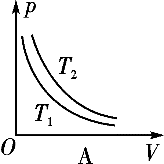
\includegraphics[width=0.74514in,height=0.74514in]{media/image495.png}
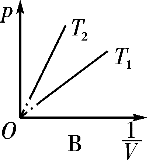
\includegraphics[width=0.70764in,height=0.74514in]{media/image496.png}
&
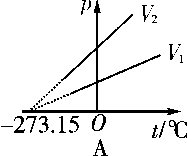
\includegraphics[width=0.84931in,height=0.70764in]{media/image497.png}
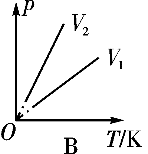
\includegraphics[width=0.67014in,height=0.69792in]{media/image498.png}
&
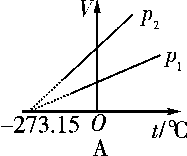
\includegraphics[width=0.84931in,height=0.70764in]{media/image499.png}
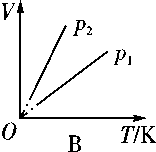
\includegraphics[width=0.70764in,height=0.68889in]{media/image500.png}
\tabularnewline
\bottomrule
\end{longtable}
\newpage
\section{热力学定律与能量守恒}


1.热力学第一定律

\ding{172}内容:一个热力学系统的\_\_内能增量\_\_等于外界向它传递的热量与外界对它所做的功的和.

\ding{173}表达式:$\Delta UQ+W$.

\ding{174}符号法则

\begin{longtable}[]{@{}llll@{}}
\toprule
符号 & W & Q & $\Delta$U\tabularnewline
\midrule
\endhead
+ & 外界对物体做功 & 物体吸收热量 &
内能增加\tabularnewline
- & 物体对外界做功 & 物体放出热量 &
内能减小\tabularnewline
\bottomrule
\end{longtable}

2.热力学第二定律的三种表述

(1)克劳修斯表述:热量不能\_\_自发地\_\_从低温物体传到高温物体.

(2)开尔文表述:不可能从\_\_单一\_\_热库吸收热量,使之完全变成功,而\_\_不产生\_\_其他影响.或表述为``第二类永动机不可能制成''.

(3)用熵的概念进行表述:在任何自然过程中,一个孤立系统的总熵不会\_\_减小\_\_(热力学第二定律又叫做熵增加原理).

3.能量守恒定律

(1)内容

能量既不会凭空产生,也不会凭空消失,它只能从一种形式\_\_转化\_\_为另一种形式,或者从一个物体\_\_转移\_\_到别的物体,在转化或转移的过程中,能量的\_\_总和\_\_保持不变.

(2)能源的利用

\ding{172}存在能量耗散和\_\_品质降低\_\_.

\ding{173}重视利用能源时对\_\_环境\_\_的影响.

\ding{174}推进开发新能源,如\_\_太阳能\_\_、生物能、风能、潮汐能等.

\newpage
\subsection{热力学第一定律}

1.改变内能的两种方式的比较

\begin{longtable}[]{@{}m{1.5cm}m{5cm}m{5cm}@{}}
\toprule
&
做功
&
热传递
\tabularnewline
\midrule
\endhead
内能变化情况
&
外界对物体做功,物体的内能增加;物体对外界做功,物体的内能减少
&
物体吸收热量,内能增加;物体放出热量,内能减少
\tabularnewline
从运动形式上看 & 做功是宏观的机械运动向物体的微观分子热运动的转化 &
热传递则是通过分子之间的相互作用,使同一物体的不同部分或不同物体间的分子热运动发生变化,是内能的转移\tabularnewline
从能量的角度看 & 做功是其他形式的能与内能相互转化的过程 &
不同物体间或同一物体不同部分之间内能的转移\tabularnewline
能的性质变化情况 & 能的性质发生了变化 & 能的性质不变\tabularnewline
相互联系 & \multicolumn{2}{c}{做一定量的功或传递一定量的热量在改变内能的效果上是相同的}
\tabularnewline
\bottomrule
\end{longtable}

2.热力学第一定律不仅反映了做功和热传递这两种改变内能的过程是等效的,而且给出了内能的变化量和做功与热传递之间的定量关系.此定律是标量式,应用时功、内能、热量的单位应统一为国际单位焦耳.

3.三种特殊情况

(1)若过程是绝热的,则$Q=0,W\neq U$,外界对物体做的功等于物体内能的增加;

(2)若过程中不做功,即$W=0,则Q\neq U$,物体吸收的热量等于物体内能的增加;

(3)若过程的始、末状态物体的内能不变,即$\Delta$U=0,则W+Q=0或W=-Q,外界对物体做的功等于物体放出的热量.

\begin{center}
\includegraphics[width=0.70764in,height=0.12292in]{media/image34.png}\end{center}
\begin{center}
    \textbf{理想气体内能变化的判定}
\end{center}

对一定质量的理想气体,由于无分子势能,其内能只包含分子无规则热运动的动能,这时内能只与温度有关,故判定一定质量的理想气体内能是否变化,应看温度是否发生了变化,与体积无关.

\newpage
\subsection{热力学第二定律}

1.热力学过程方向性实例

(1)高温物体$\xlongrightarrow[\text{热量Q不能自发传给}]{\text{ 热量Q能自发传给}}$低温物体

(2)功$\xlongrightarrow[\text{不能自发地且不能完全转化为}]{\text{能自发地完全转化为}}$热量

(3)气体体积$V_1$$\xlongrightarrow[\text{不能自发收缩到}]{\text{能自发膨胀到}}$气体体积$V_2$(较大)

(4)不同气体A和B$\xlongrightarrow[\text{不能自发分离成}]{\text{能自发混合成}}$混合气体AB

2.热力学第一定律和热力学第二定律的关系

热力学第一定律是和热现象有关的物理过程中能量守恒的特殊表达形式及热量与内能改变的定量关系.而第二定律指明了能量转化与守恒能否实现的条件和过程进行的方向,指出了一切变化过程的自然发展是不可逆的,除非靠外界影响.所以二者相互联系,又相互补充.

3.两类永动机的比较

\begin{longtable}[]{@{}m{5cm}m{5cm}@{}}
\toprule
第一类永动机 & 第二类永动机\tabularnewline
\midrule
\endhead
不消耗能量却可以源源不断地对外做功的机器 &
从单一热源吸热,全部用来对外做功而不引起其他变化的机器\tabularnewline
违背能量守恒,不可能实现 &
不违背能量守恒,违背热力学第二定律,不可能实现\tabularnewline
\bottomrule
\end{longtable}


\begin{center}
\includegraphics[width=0.70764in,height=0.12292in]{media/image13.png}\end{center}
\begin{center}
    \textbf{热力学第二定律的涵义}
\end{center}

(1)``自发地''指明了热传递等热力学宏观现象的方向性,不需要借助外界提供能量的帮助.

(2)``不产生其他影响''的含义是发生的热力学宏观过程只在本系统内完成,对周围环境不产生热力学方面的影响,如吸热、放热、做功等.
